\documentclass[aspectratio=169,11pt]{beamer}

% Shared presentation style, adapted from reference-slides/.
\usetheme[progressbar=frametitle,numbering=fraction]{metropolis}

\usepackage[T1]{fontenc}
\usepackage{amsmath,amssymb}
\usepackage{booktabs}
\usepackage{braket}
\usepackage{microtype}
\usepackage{tabularx}
\usepackage{tikz}
\usepackage{qcircuit}
% Classical gate from the paper; this qcircuit version provides only \gate.
\providecommand{\cgate}[1]{*+<.6em>{#1} \POS ="i","i"+UR;"i"+UL
  **\dir{-};"i"+DL **\dir{-};"i"+DR **\dir{-};"i"+UR **\dir{-},"i" \cw}
\usepackage{pgfpages}
\usetikzlibrary{arrows.meta,calc,decorations.pathreplacing,fit,positioning}

% Notes stay in the source; `make notes` places them on a second screen.
\ifdefined\showspeakernotes
  \setbeameroption{show notes on second screen=right}
  % Avoid duplicate PDF destinations when pgfpages composes the two screens.
  \hypersetup{draft}
\else
  \setbeameroption{hide notes}
\fi

% Palette and typography match the reference presentation.
\definecolor{CVQCInk}{HTML}{17324D}
\definecolor{CVQCTeal}{HTML}{087E8B}
\definecolor{CVQCPale}{HTML}{E8F3F4}
\definecolor{CVQCGold}{HTML}{E5A23B}
\definecolor{CVQCGoldPale}{HTML}{FFF2D8}
\definecolor{CVQCCoral}{HTML}{C85151}
\definecolor{CVQCCoralPale}{HTML}{F9E8E6}
\definecolor{CVQCMuted}{HTML}{5E6D78}
\definecolor{CVQCFog}{HTML}{F4F7F8}

\setbeamercolor{normal text}{fg=CVQCInk,bg=white}
\setbeamercolor{alerted text}{fg=CVQCCoral}
\setbeamercolor{example text}{fg=CVQCTeal}
\setbeamercolor{frametitle}{fg=white,bg=CVQCInk}
\setbeamercolor{progress bar}{fg=CVQCTeal,bg=CVQCPale}
\setbeamercolor{progress bar in head/foot}{fg=CVQCTeal,bg=CVQCPale}
\setbeamercolor{title separator}{fg=CVQCTeal}
\setbeamercolor{palette primary}{fg=white,bg=CVQCInk}
\setbeamercolor{block title}{fg=white,bg=CVQCInk}
\setbeamercolor{block body}{fg=CVQCInk,bg=CVQCFog}
\setbeamercolor{block title alerted}{fg=white,bg=CVQCCoral}
\setbeamercolor{block body alerted}{fg=CVQCInk,bg=CVQCCoralPale}
\setbeamercolor{block title example}{fg=white,bg=CVQCTeal}
\setbeamercolor{block body example}{fg=CVQCInk,bg=CVQCPale}
\setbeamercolor{takeaway}{fg=CVQCInk,bg=CVQCPale}
\setbeamercolor{question}{fg=CVQCInk,bg=CVQCGoldPale}

\setbeamerfont{title}{series=\bfseries,size=\huge}
\setbeamerfont{frametitle}{series=\bfseries,size=\Large}
\setbeamerfont{block title}{series=\bfseries}
\setbeamertemplate{navigation symbols}{}
\metroset{block=fill}

% An atom marks a quantum party, as in Hung's QCrypt 2020 talk, p. 10:
% https://2020.qcrypt.net/slides/QCrypt2020TalkSlides058Hung.pdf
% Draw inside the party's scope so the marker follows its diagram scale.
\newcommand{\quantumpartymark}[1]{%
  \begin{scope}[shift={($(#1.north east)+(0.15,0.3)$)},
      draw=CVQCTeal,line width=1.1pt]
    \foreach \angle in {0,60,120} {
      \draw[rotate=\angle] (0,0) ellipse[x radius=0.58cm,y radius=0.21cm];
    }
    \fill[CVQCGold] (0,0) circle[radius=0.075cm];
    \fill[CVQCTeal] (0.58,0) circle[radius=0.045cm];
  \end{scope}%
}

% Reusable callouts for later slides.
\newcommand{\takeaway}[1]{%
  \begin{beamercolorbox}[wd=\textwidth,sep=0.85ex,rounded=true,center]{takeaway}
    #1
  \end{beamercolorbox}%
}
\newcommand{\questionbox}[1]{%
  \begin{beamercolorbox}[wd=\textwidth,sep=1ex,rounded=true,center]{question}
    #1
  \end{beamercolorbox}%
}


% Title follows CVQC-paper/paper-title.tex; authors match the STOC submission.
% Yi Lee is underlined as the speaker, following the reference talk.
\title[Classical Verification of Quantum Sampling]{%
  \texorpdfstring{%
    Classical Verification of\\
    Quantum Sampling\\
    with Negligible Error%
  }{Classical Verification of Quantum Sampling with Negligible Error}}
\author[Chung, Cojocaru, Lee, Lin]{%
  \texorpdfstring{%
    Kai-Min Chung\textsuperscript{1}\quad
    Alexandru Cojocaru\textsuperscript{2}\quad
    \underline{Yi Lee}\textsuperscript{3}\\[0.3em]
    Han-Hsuan Lin\textsuperscript{4}%
  }{Kai-Min Chung, Alexandru Cojocaru, Yi Lee, Han-Hsuan Lin}}
\institute{%
  \textsuperscript{1}Academia Sinica\quad
  \textsuperscript{2}University of Edinburgh\quad
  \textsuperscript{3}University of Maryland\\[0.25em]
  \textsuperscript{4}National Tsing Hua University}
% Set the occasion/date here when known; leave blank for now.
\date{}

\begin{document}

\begin{frame}[plain]
  \vfill
  {\usebeamerfont{title}\color{CVQCInk}\inserttitle\par}
  \vspace{0.8em}
  {\color{CVQCTeal}\rule{0.48\textwidth}{1.2pt}\par}

  \vspace{1.2em}
  {\small\bfseries\insertauthor\par}
  \vspace{1em}
  {\scriptsize\color{CVQCMuted}\insertinstitute\par}

  \vfill
  {\footnotesize\bfseries\color{CVQCGold}\insertdate\par}
\end{frame}

% outline.md, lines 9--35: one frame with five successive overlays.
\begin{frame}{Classical Verification of Quantum Computation}
  \centering
  \begin{tikzpicture}[
      >={Latex[length=3mm]},
      party/.style={circle,draw=CVQCInk,fill=CVQCFog,very thick,
        minimum size=2.5cm,text width=2.1cm,inner sep=0pt,
        align=center,font=\large\bfseries,text=CVQCInk},
      callout/.style={fill=CVQCPale,rounded corners=4mm,
        minimum width=4.7cm,minimum height=0.95cm,
        align=center,text=CVQCInk,inner sep=3mm},
      communication/.style={->,line width=1.5pt,draw=CVQCTeal}
    ]
    % Reserve the same space on every overlay so the parties never move.
    \path[use as bounding box] (-6.5,-2.85) rectangle (6.5,3.1);

    \node[party] (verifier) at (-4.15,0) {Verifier};
    \node[party,fill=CVQCPale] (prover) at (4.15,0) {Prover};
    \quantumpartymark{prover}

    % Pale bubbles and angled tails follow Mending-Slides/diagrams/results.tex.
    % Each annotation belongs only to its own stage of the interaction.
    % Input and output share a raised bubble, giving its tail a gentler angle.
    \only<2,4-5>{
      \node[callout] (annotation) at (-3.15,2.45) {};
      \path[fill=CVQCPale]
        ($(annotation.south)+(-0.65,0.02)$) --
        ($(verifier.north)+(-0.15,0.06)$) --
        ($(annotation.south)+(-0.05,0.02)$) -- cycle;
      \node[font=\large,text=CVQCInk] at (annotation.center) {%
        \only<2>{$C(x)$: Quantum circuit}%
        \only<4>{$y$: circuit output}%
        \only<5>{$y \gets C(x)\;\text{or}\;\textcolor{CVQCCoral}{\mathsf{reject}}$}%
      };
    }

    \only<3>{
      % Leave a gap to both circles, even at their widest point.
      \draw[communication] (-2.35, 1.10) -- ( 2.35, 1.10);
      \draw[communication] ( 2.35, 0.50) -- (-2.35, 0.50);
      \draw[communication] (-2.35,-0.10) -- ( 2.35,-0.10);
      \node[font=\large,text=CVQCTeal] at (0,-0.60) {$\vdots$};
      \draw[communication] ( 2.35,-1.10) -- (-2.35,-1.10);
    }

  \end{tikzpicture}

  \note<1>{
    \footnotesize
    Think of a classical client using a remote quantum server. The server can
    perform computations beyond the client's reach, but how can the client
    check that the computation was performed correctly? This is also a natural
    question when demonstrating quantum advantage: the very separation that
    makes the computation interesting makes its output difficult to verify.
  }
  \note<2>{
    \footnotesize
    The client has a description of a quantum circuit $C$ and a classical input
    $x$. Here $C(x)$ denotes running that circuit and measuring its output to
    obtain a classical sample. Knowing the circuit does not mean the client can
    efficiently execute it.
  }
  \note<3>{
    \footnotesize
    The verifier and prover exchange classical messages. The alternating
    arrows and ellipsis stand for an interactive protocol, potentially with
    many rounds; the arrows are schematic, not an exact message count.
    The verifier remains entirely classical; the prover does the quantum work.
  }
  \note<4>{
    \footnotesize
    At the end, the verifier produces a classical output $y$. The goal is to
    verify this output through the interaction, without having to reproduce
    the quantum computation locally.
  }
  \note<5>{
    \footnotesize
    This is shorthand for the desired sample-or-reject behavior, up to the
    protocol's error. Completeness: an honest prover makes the verifier accept
    and return a sample from $C(x)$ with high probability. Soundness: even an
    efficient cheating prover cannot make the verifier's output distinguishable
    from an ideal experiment that independently samples from $C(x)$ or rejects.
    The ideal experiment has the same acceptance probability as the real one.
    The guarantee concerns the entire output distribution, including rejection;
    a single sample is not individually classified as correct or incorrect.
  }
\end{frame}

% Smaller copies of the message diagram from slides/02-cvqc.tex.
% Arguments: vertical position, verifier label.
\newcommand{\strategyprotocol}[2]{%
  \begin{scope}[shift={(0,#1)},scale=0.68,transform shape]
    \node[party] at (-4.15,0) {#2};
    \node[party] at (4.15,0) {Prover};

    \draw[communication] (-2.35, 1.10) -- ( 2.35, 1.10);
    \draw[communication] ( 2.35, 0.50) -- (-2.35, 0.50);
    \draw[communication] (-2.35,-0.10) -- ( 2.35,-0.10);
    \node[font=\large,text=CVQCTeal] at (0,-0.60) {$\vdots$};
    \draw[communication] ( 2.35,-1.10) -- (-2.35,-1.10);
  \end{scope}%
}

% outline.md, lines 37--45.
\begin{frame}{CVQC Strategy}
  \centering
  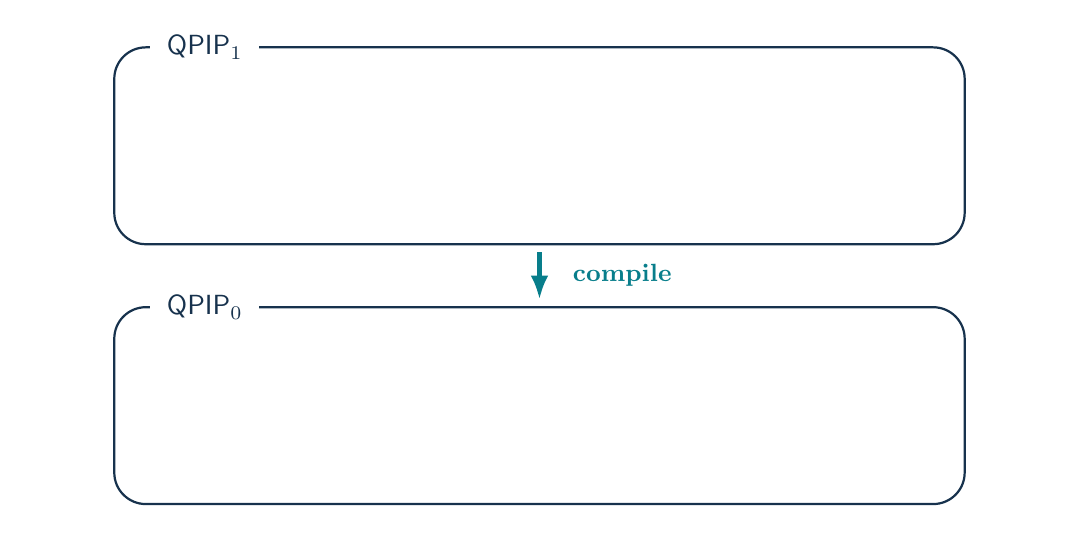
\begin{tikzpicture}[
      >={Latex[length=3mm]},
      party/.style={circle,draw=CVQCInk,fill=CVQCFog,very thick,
        minimum size=2.5cm,text width=2.1cm,inner sep=0pt,
        align=center,font=\large\bfseries,text=CVQCInk},
      communication/.style={->,line width=1.5pt,draw=CVQCTeal},
      protocolbox/.style={draw=CVQCInk,thick,rounded corners=4mm},
      modellabel/.style={fill=white,inner xsep=6pt,inner ysep=2pt,
        font=\bfseries,text=CVQCInk}
    ]
    % Keep the first diagram in place when revealing the compiler below it.
    \path[use as bounding box] (-6.5,-3.15) rectangle (6.5,3.15);

    \draw[protocolbox] (-5.4,0.4) rectangle (5.4,2.9);
    \node[modellabel] at (-4.25,2.9) {$\mathsf{QPIP}_1$};
    \strategyprotocol{1.65}{Weak\\quantum\\verifier}

    \only<2>{
      \draw[->,line width=1.5pt,draw=CVQCTeal] (0,0.30) -- (0,-0.30)
        node[midway,right=8pt,font=\small\bfseries,text=CVQCTeal] {compile};

      \draw[protocolbox] (-5.4,-2.9) rectangle (5.4,-0.4);
      \node[modellabel] at (-4.25,-0.4) {$\mathsf{QPIP}_0$};
      \strategyprotocol{-1.65}{Classical\\verifier}
    }
  \end{tikzpicture}

  \note<1>{
    \footnotesize
    A common strategy is to begin with a verifier that has a small amount of
    quantum capability, interacting with a full quantum prover. We refer to
    this model as $\mathsf{QPIP}_1$. In our construction, the verifier only
    prepares and sends individual qubits from a fixed finite set; the rest of
    the interaction is classical. The arrows indicate interaction, not a
    particular number of messages.
  }
  \note<2>{
    \footnotesize
    Next, compile the protocol to remove the verifier's quantum operations,
    giving a fully classical verifier interacting with the quantum prover:
    the $\mathsf{QPIP}_0$ model. The bottom protocol is the compiled version
    of the one above. This is the overall strategy; the next slides show
    two paradigms for implementing this compilation. In our prepare-and-send setting, the
    quantum preparation is replaced with remote state preparation.
  }
\end{frame}

% Same geometry as the strategy slide, focusing on quantum preparation.
% Arguments: vertical position, verifier label, arrow label.
\newcommand{\preparesendprotocol}[3]{%
  \begin{scope}[shift={(0,#1)},scale=0.68,transform shape]
    \node[party] at (-4.15,0) {#2};
    \node[party] at (4.15,0) {Prover};
    \draw[communication] (-2.35,0) --
      node[above=7pt,align=center,font=\large,text=CVQCInk] {#3}
      (2.35,0);
  \end{scope}%
}

% outline.md, lines 47--52.
\begin{frame}{CVQC Strategy: Prepare-and-Send}
  \centering
  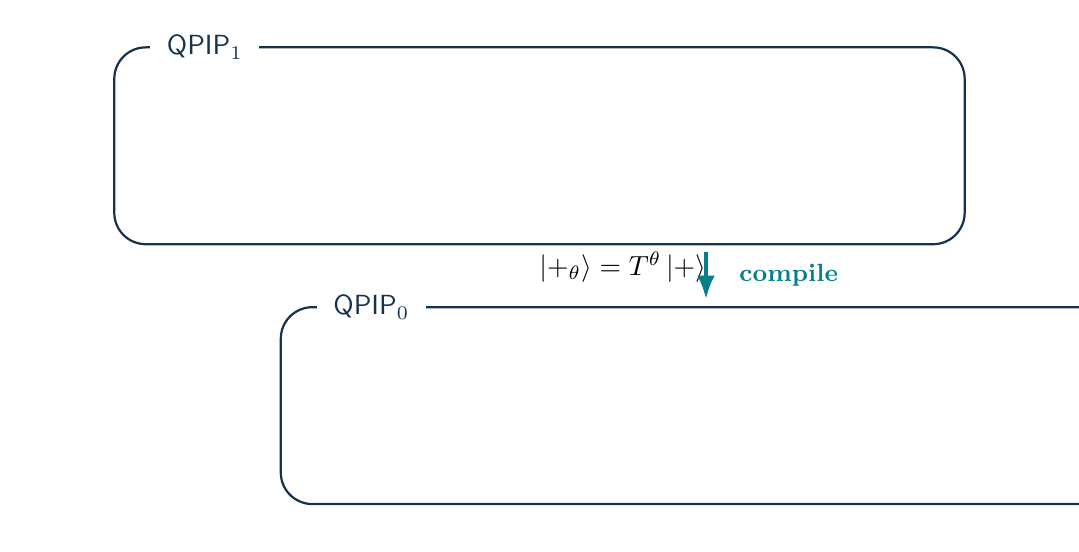
\begin{tikzpicture}[
      >={Latex[length=3mm]},
      party/.style={circle,draw=CVQCInk,fill=CVQCFog,very thick,
        minimum size=2.5cm,text width=2.1cm,inner sep=0pt,
        align=center,font=\large\bfseries,text=CVQCInk},
      communication/.style={->,line width=1.5pt,draw=CVQCTeal},
      protocolbox/.style={draw=CVQCInk,thick,rounded corners=4mm},
      modellabel/.style={fill=white,inner xsep=6pt,inner ysep=2pt,
        font=\bfseries,text=CVQCInk}
    ]
    \path[use as bounding box] (-6.5,-3.15) rectangle (6.5,3.15);

    \draw[protocolbox] (-5.4,0.4) rectangle (5.4,2.9);
    \node[modellabel] at (-4.25,2.9) {$\mathsf{QPIP}_1$};
    \preparesendprotocol{1.65}{Weak\\quantum\\verifier}%
      {$\ket{+_{\theta}}=T^{\theta}\ket{+}$}

    \only<2>{
      \draw[->,line width=1.5pt,draw=CVQCTeal] (0,0.30) -- (0,-0.30)
        node[midway,right=8pt,font=\small\bfseries,text=CVQCTeal] {compile};

      \draw[protocolbox] (-5.4,-2.9) rectangle (5.4,-0.4);
      \node[modellabel] at (-4.25,-0.4) {$\mathsf{QPIP}_0$};
      \preparesendprotocol{-1.65}{Classical\\verifier}{Remote state\\preparation}
    }
  \end{tikzpicture}

  \note<1>{
    \footnotesize
    In the prepare-and-send paradigm, the weak quantum verifier prepares
    single-qubit states and sends them to the prover. For example,
    $\ket{+_{\theta}}=T^{\theta}\ket{+}
    =(\ket{0}+e^{i\pi\theta/4}\ket{1})/\sqrt{2}$, where
    $T=\operatorname{diag}(1,e^{i\pi/4})$ and
    $\theta\in\mathbb{Z}_8$ is chosen by the verifier, following the paper's
    angle convention. The picture focuses on these quantum messages;
    the rest of the classical interaction is left implicit.
  }
  \note<2>{
    \footnotesize
    Replace the quantum preparation and transmission with remote state
    preparation: a classical interaction that leaves the prover holding a
    quantum state correlated with the verifier's classical information.
    The lower arrow represents this interactive subprotocol, rather than a
    single classical message. This gives the overall prepare-and-send route
    to a fully classical verifier; we will discuss the required guarantees
    and our particular construction later.
  }
\end{frame}

% Same geometry as prepare-and-send, with the quantum message reversed.
% Optional verifier decoration; arguments: vertical position, verifier/arrow labels.
\newcommand{\receivemeasureprotocol}[4][]{%
  \begin{scope}[shift={(0,#2)},scale=0.68,transform shape]
    \node[party] (verifier) at (-4.15,0) {#3};
    #1%
    \node[party,fill=CVQCPale] (prover) at (4.15,0) {Prover};
    \quantumpartymark{prover}
    \draw[communication] (2.35,0) --
      node[above=7pt,align=center,font=\large,text=CVQCInk] {#4}
      (-2.35,0);
  \end{scope}%
}

% outline.md, lines 54--58.
\begin{frame}{CVQC Strategy: Receive-and-Measure}
  \centering
  \begin{tikzpicture}[
      >={Latex[length=3mm]},
      party/.style={circle,draw=CVQCInk,fill=CVQCFog,very thick,
        minimum size=2.5cm,text width=2.1cm,inner sep=0pt,
        align=center,font=\large\bfseries,text=CVQCInk},
      communication/.style={->,line width=1.5pt,draw=CVQCTeal},
      protocolbox/.style={draw=CVQCInk,thick,rounded corners=4mm},
      modellabel/.style={fill=white,inner xsep=6pt,inner ysep=2pt,
        font=\bfseries,text=CVQCInk}
    ]
    \path[use as bounding box] (-6.5,-3.15) rectangle (6.5,3.15);

    \draw[protocolbox] (-5.4,0.4) rectangle (5.4,2.9);
    \node[modellabel] at (-4.25,2.9) {$\mathsf{QPIP}_1$};
    \receivemeasureprotocol[\quantumpartymark{verifier}]{1.65}{Weak\\quantum\\verifier}%
      {$\ket{\psi_{\mathrm{hist}}}$}

    \only<2>{
      \draw[->,line width=1.5pt,draw=CVQCTeal] (0,0.30) -- (0,-0.30)
        node[midway,right=8pt,font=\small\bfseries,text=CVQCTeal] {compile};

      \draw[protocolbox] (-5.4,-2.9) rectangle (5.4,-0.4);
      \node[modellabel] at (-4.25,-0.4) {$\mathsf{QPIP}_0$};
      \receivemeasureprotocol{-1.65}{Classical\\verifier}{Commit-and-measure}
    }
  \end{tikzpicture}

  \note<1>{
    \footnotesize
    The other paradigm reverses the quantum communication. The prover supplies
    a history state encoding the computation, and the weak quantum verifier
    checks it using simple measurements. The picture suppresses the classical
    interaction and the details of the history-state test.
  }
  \note<2>{
    \footnotesize
    Replace receiving and measuring the state with a classical
    commit-and-measure protocol. The prover commits to a quantum state, and the
    verifier uses classical interaction to obtain certified measurement
    outcomes. The arrow represents this functionality, not a single message.
    This is the route exemplified by Mahadev's measurement protocol.
    Source: \href{https://arxiv.org/abs/1804.01082}{Urmila Mahadev,
    Classical Verification of Quantum Computations (FOCS 2018)}.
  }
\end{frame}

% Fixed columns keep the table stable as rows appear.
% Arguments: vertical position, work, paradigm, task, soundness error.
\newcommand{\surveyrow}[5]{%
  \node[tablecell] at (-6.45,#1) {#2};
  \node[tablecell] at (-2.75,#1) {#3};
  \node[tablecell] at ( 1.05,#1) {#4};
  \node[tablecell] at ( 3.40,#1) {#5};
}

% outline.md, lines 60--75. References link directly to the papers.
\begin{frame}{Literature Survey}
  \centering
  \begin{tikzpicture}[
      tablecell/.style={anchor=west,inner sep=0pt,font=\small,text=CVQCInk},
      tablehead/.style={tablecell,font=\small\bfseries},
      separator/.style={draw=CVQCMuted!25,line width=0.4pt}
    ]
    \path[use as bounding box] (-6.7,-3.0) rectangle (6.7,2.9);

    \node[tablehead] at (-6.45,2.45) {Work};
    \node[tablehead] at (-2.75,2.45) {Paradigm};
    \node[tablehead] at ( 1.05,2.45) {Problem type};
    \node[tablehead] at ( 3.40,2.45) {Soundness error};
    \draw[draw=CVQCInk,line width=0.8pt] (-6.65,2.10) -- (6.65,2.10);

    \surveyrow{1.65}%
      {[\href{https://arxiv.org/abs/1904.06320}{GV19},
        \href{https://drops.dagstuhl.de/entities/document/10.4230/LIPIcs.ICALP.2023.67}{GMP23},
        \href{https://arxiv.org/abs/2609.38060}{HN26}]}%
      {Prepare-and-send}{Decision}{Negligible}

    \only<2->{
      \draw[separator] (-6.65,1.23) -- (6.65,1.23);
      \surveyrow{0.80}%
        {[\href{https://arxiv.org/abs/1804.01082}{Mah18},
          \href{https://arxiv.org/abs/1912.00990}{CCY20}]}%
        {Receive-and-measure}{Decision}{Negligible}
    }

    \only<3->{
      \draw[separator] (-6.65,0.38) -- (6.65,0.38);
      \surveyrow{-0.05}%
        {[\href{https://arxiv.org/abs/2012.04848}{CLLW22}]}%
        {Receive-and-measure}{Sampling}{Inverse-polynomial}
    }

    \only<4->{
      \fill[CVQCPale,rounded corners=3pt] (-6.65,-1.28) rectangle (6.65,-0.52);
      \begin{scope}[tablecell/.append style={font=\small\bfseries,text=CVQCTeal}]
        \surveyrow{-0.90}{This work}{Prepare-and-send}{Sampling}{Negligible}
      \end{scope}
    }

    \only<5>{
      \surveyrow{-1.75}%
        {[\href{https://arxiv.org/abs/2610.31775}{KKR26}]}%
        {Receive-and-measure}{Sampling}{Negligible}
    }

  \end{tikzpicture}

  \note<1>{
    \footnotesize
    Representative results, grouped by the two paradigms rather than an
    exhaustive chronology. GV19 is Alexandru Gheorghiu and Thomas Vidick,
    Computationally-secure and composable remote state preparation (FOCS 2019).
    GMP23 is Alexandru Gheorghiu, Tony Metger, and Alexander Poremba,
    Quantum Cryptography with Classical Communication (ICALP 2023).
    HN26 is Finn Holler and Anand Natarajan, Classical Verification of Quantum
    Computation with Quasilinear Resources, from Compiled Nonlocal Games (2026).
    They use a computational self-test and remote preparation to compile
    Broadbent's protocol, achieving quasilinear total resources under
    subexponential LWE hardness. Their stated BQP theorem has a constant gap.
    All three use remote preparation to remove quantum messages from the verifier.
    The negligible-error entry refers to decision verification after
    amplification. The preparation primitives have their own approximation
    guarantees; this row does not claim negligible-error remote preparation.
  }
  \note<2>{
    \footnotesize
    Mah18 is Urmila Mahadev, Classical Verification of Quantum Computations
    (FOCS 2018). CCY20 is Nai-Hui Chia, Kai-Min Chung, and Takashi Yamakawa,
    Classical Verification of Quantum Computations with Efficient Verifier
    (TCC 2020). The latter proves negligible soundness for parallel repetition
    of Mahadev's protocol. The table records the amplified decision guarantee,
    not the soundness of a single run of the original protocol.
  }
  \note<3>{
    \footnotesize
    CLLW22 is Kai-Min Chung, Yi Lee, Han-Hsuan Lin, and Xiaodi Wu,
    Constant-Round Blind Classical Verification of Quantum Sampling
    (EUROCRYPT 2022). It extends the Mahadev approach to sampling, but with
    inverse-polynomial soundness error. A majority vote that amplifies a
    decision bit does not generically turn several imperfect samples into a
    sample from the desired distribution. Soundness here concerns the whole
    sample-or-reject output distribution.
  }
  \note<4>{
    \footnotesize
    Our work follows the prepare-and-send route and achieves negligible
    soundness error for sampling. Emphasize the difference from the preceding
    row: the problem type stays sampling, while the soundness error becomes
    negligible. The next slide will separate our weak-quantum-verifier result
    from the fully classical compilation and state their assumptions.
  }
  \note<5>{
    \footnotesize
    KKR26 is Yael Tauman Kalai, Dakshita Khurana, and Justin Raizes,
    \href{https://arxiv.org/abs/2610.31775}{The Entire Quantum Computer on a
    Classical Leash (2026)}. This is concurrent and independent work, identified
    in the talk outline as STOC submission 598. Their framework builds on
    committed history states and non-destructive testing, and obtains
    negligible-error sampling verification under post-quantum LWE. The
    receive-and-measure label describes that underlying route; their full
    construction provides a more general classical--quantum two-party
    computation functionality.
  }
\end{frame}

% outline.md, lines 77--81: two results in the familiar compilation layout.
\begin{frame}{Main Contributions}
  \centering
  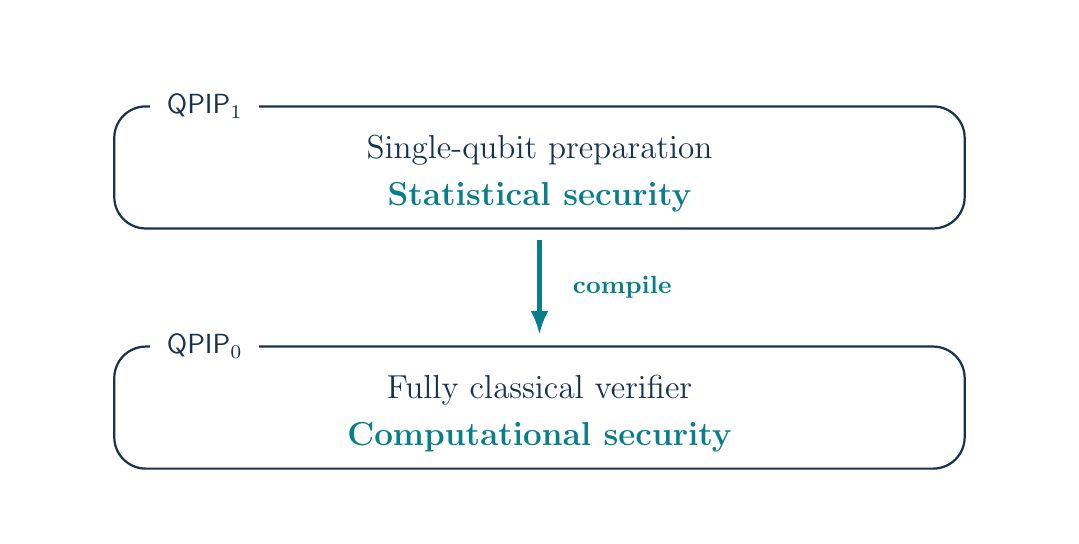
\begin{tikzpicture}[
      >={Latex[length=3mm]},
      resultcard/.style={draw=CVQCInk,thick,rounded corners=4mm},
      modellabel/.style={fill=white,inner xsep=6pt,inner ysep=2pt,
        font=\bfseries,text=CVQCInk},
      capability/.style={font=\large,text=CVQCInk},
      guarantee/.style={font=\large\bfseries,text=CVQCTeal}
    ]
    \path[use as bounding box] (-6.5,-3.1) rectangle (6.5,3.1);

    \draw[resultcard] (-5.4,0.55) rectangle (5.4,2.10);
    \node[modellabel] at (-4.25,2.10) {$\mathsf{QPIP}_1$};
    \node[capability] at (0,1.55) {Single-qubit preparation};
    \node[guarantee] at (0,0.95) {Statistical security};

    \only<2>{
      \draw[->,line width=1.5pt,draw=CVQCTeal] (0,0.40) -- (0,-0.80)
        node[midway,right=8pt,font=\small\bfseries,text=CVQCTeal] {compile};

      \draw[resultcard] (-5.4,-2.50) rectangle (5.4,-0.95);
      \node[modellabel] at (-4.25,-0.95) {$\mathsf{QPIP}_0$};
      \node[capability] at (0,-1.50) {Fully classical verifier};
      \node[guarantee] at (0,-2.10) {Computational security};
    }
  \end{tikzpicture}

  \note<1>{
    \footnotesize
    Our first contribution is a protocol for verifying arbitrary efficient
    quantum sampling computations with negligible soundness error, using a
    verifier that only prepares and sends single qubits from a fixed finite
    set. The guarantee is statistical and holds even against an unbounded
    prover, without computational assumptions. All subsequent interaction is
    classical. This is a result in its own right, as well as the foundation of
    the fully classical protocol.
  }
  \note<2>{
    \footnotesize
    For now, describe the compilation in words. Introduce classical-client
    QFHE and its role later, with the remote preparation construction.
    Our second contribution removes the verifier's quantum capability,
    assuming subexponentially quantum-secure classical-client QFHE. We use
    Holler--Natarajan's computational self-testing machinery for remote
    preparation, together with our analysis of the prepared resources and
    authenticated distillation. The resulting classical-verifier protocol
    has negligible computational soundness error for sampling. Both results
    concern the full sample-or-reject output distribution, compared with an
    ideal experiment having the same acceptance probability.
    Next, introduce distillation and quantum authentication before explaining
    the construction.
  }
\end{frame}

% Motivate error reduction before introducing the distillation picture.
\begin{frame}{Error Reduction}
  \centering
  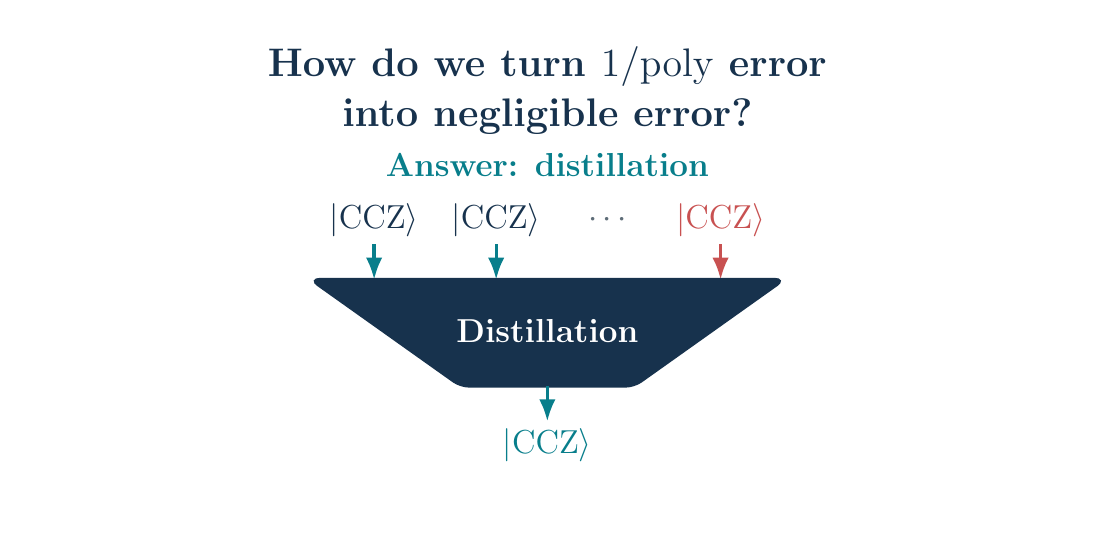
\begin{tikzpicture}[
      >={Latex[length=2.8mm]},
      questiontitle/.style={font=\Large\bfseries,text=CVQCInk,align=center},
      resource/.style={font=\large,text=CVQCInk},
      flow/.style={->,very thick,draw=CVQCTeal}
    ]
    \path[use as bounding box] (-6.6,-3.15) rectangle (6.6,3.05);

    % Keep the question fixed; the second overlay only adds the answer.
    \node[questiontitle] at (0,2.25)
      {How do we turn $1/\mathrm{poly}$ error\\into negligible error?};

    \only<2>{
      \node[font=\large\bfseries,text=CVQCTeal] at (0,1.30) {Answer: distillation};
      \begin{scope}[yshift=-0.3cm]
        \node[resource] at (-2.20,0.90) {$\ket{\mathrm{CCZ}}$};
        \node[resource] at (-0.65,0.90) {$\ket{\mathrm{CCZ}}$};
        \node[font=\large,text=CVQCMuted] at (0.80,0.90) {$\cdots$};
        \node[resource,text=CVQCCoral] at (2.20,0.90) {$\ket{\mathrm{CCZ}}$};

        \draw[flow] (-2.20,0.60) -- (-2.20,0.15);
        \draw[flow] (-0.65,0.60) -- (-0.65,0.15);
        \draw[flow,draw=CVQCCoral] (2.20,0.60) -- (2.20,0.15);

        % Wide top, narrow bottom: a schematic distillation funnel.
        \path[draw=CVQCInk,fill=CVQCInk,very thick,rounded corners=3pt]
          (-3.00,0.15) -- (3.00,0.15) -- (1.10,-1.20) -- (-1.10,-1.20) -- cycle;
        \node[font=\large\bfseries,text=white] at (0,-0.50) {Distillation};

        \draw[flow] (0,-1.20) -- (0,-1.65);
        \node[resource,text=CVQCTeal] at (0,-1.95) {$\ket{\mathrm{CCZ}}$};
      \end{scope}
    }
  \end{tikzpicture}

  \note<1>{
    \footnotesize
    The goal is to reduce inverse-polynomial verification error to negligible
    error with polynomial resources. For decision problems, repetition and
    majority vote can amplify a decision bit. There is no generic majority
    vote for samples that preserves their target distribution. Our approach
    reduces errors in the quantum resources before producing the final sample.
    This motivates our construction; it is not a generic amplification theorem
    for an arbitrary sampling-verification protocol.
  }
  \note<2>{
    \footnotesize
    Distillation combines many imperfect quantum resource states to obtain a
    cleaner surviving resource, conditioned on successful checks. The picture
    uses $\ket{\mathrm{CCZ}}$ as an example; the state symbols indicate the
    intended resource, and red indicates a faulty copy. The inputs must have
    sufficiently sparse errors of the kind covered by the distillation
    analysis. This picture does not assume independent errors, and does not
    promise to purify arbitrary garbage. For now, assume the distillation
    procedure is executed honestly. The details of the error reduction come
    later in the construction and analysis.
  }
\end{frame}

% One diagram; the key and security guarantee are explained in the notes.
\begin{frame}{Background: Quantum Authentication}
  \centering
  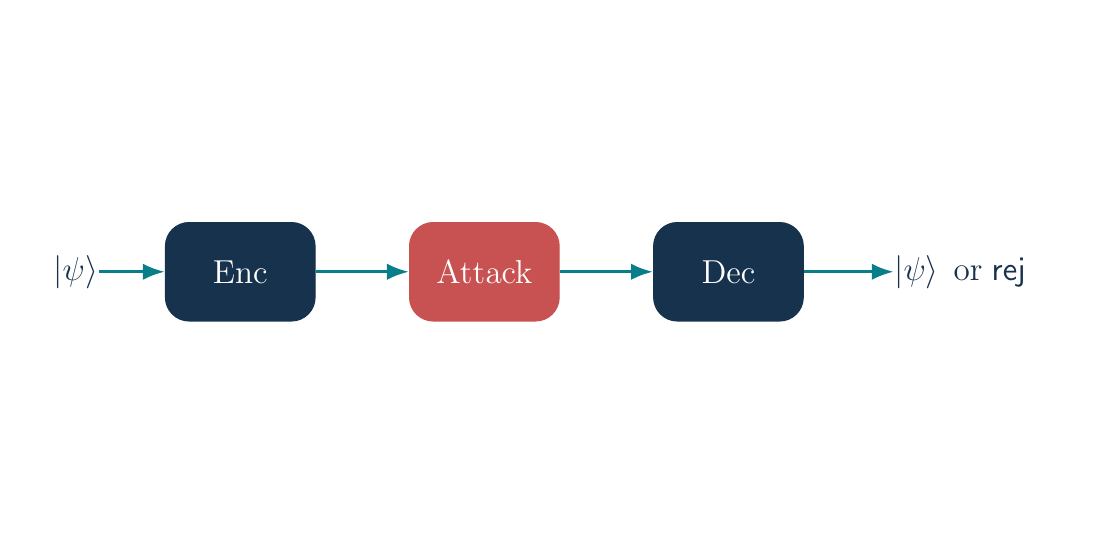
\begin{tikzpicture}[
      >={Latex[length=2.8mm]},
      process/.style={draw=CVQCInk,fill=CVQCInk,rounded corners=3mm,
        minimum width=1.9cm,minimum height=1.25cm,
        text=white,font=\large,align=center},
      attack/.style={process,draw=CVQCCoral,fill=CVQCCoral},
      flow/.style={->,very thick,draw=CVQCTeal}
    ]
    \path[use as bounding box] (-6.6,-3.1) rectangle (6.6,3.1);

    \node[anchor=east,inner sep=0pt,font=\large,text=CVQCInk]
      (input) at (-5.7,0) {$\ket{\psi}$};
    \node[process] (enc) at (-3.9,0) {$\operatorname{Enc}$};
    \node[attack] (adversary) at (-0.8,0) {Attack};
    \node[process] (dec) at (2.3,0) {$\operatorname{Dec}$};
    \node[anchor=west,inner sep=0pt,font=\large,text=CVQCInk]
      (output) at (4.4,0) {$\ket{\psi}\;\text{or}\;\mathsf{rej}$};

    \draw[flow] (input.east) -- (enc.west);
    \draw[flow] (enc.east) -- (adversary.west);
    \draw[flow] (adversary.east) -- (dec.west);
    \draw[flow] (dec.east) -- (output.west);
  \end{tikzpicture}

  \note{
    \footnotesize
    This is a symmetric-key quantum authentication scheme: encoding and
    verified decryption use the same secret key. Enc means authenticated
    encoding; Dec includes verification. Without tampering, decryption returns
    the input. The attack can be any quantum operation with private memory.
    The pure-state notation is schematic; security also preserves entanglement
    with an external reference. Undetected changes have negligible total
    weight, averaged over the key, rather than a guarantee conditioned on
    arbitrarily rare acceptance. An attacker can always force rejection.
    Authentication preserves the plaintext that was authenticated; it does not
    certify that a prepared resource is a correct CCZ state. This is the generic
    primitive; the protocol later explains how our verifier obtains and uses
    authenticated resources. Next, show the trap code. Source:
    \href{https://arxiv.org/abs/1607.03075}{Broadbent--Wainewright (2016)}.
  }
\end{frame}

% Encode and add traps, then hide them. Explain decryption verbally.
\begin{frame}{Background: The Trap Code}
  \centering
  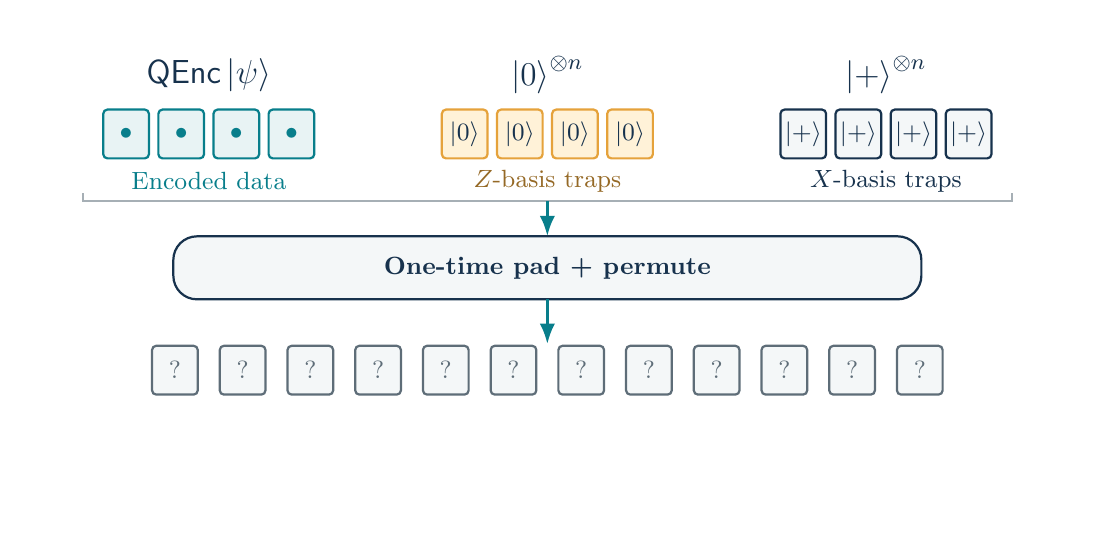
\begin{tikzpicture}[
      >={Latex[length=2.6mm]},
      qubit/.style={rounded corners=1.5pt,minimum width=0.58cm,
        minimum height=0.62cm,inner sep=1pt,font=\small,thick},
      data/.style={qubit,draw=CVQCTeal,fill=CVQCPale,text=CVQCTeal},
      ztrap/.style={qubit,draw=CVQCGold,fill=CVQCGoldPale,text=CVQCInk},
      xtrap/.style={qubit,draw=CVQCInk,fill=CVQCFog,text=CVQCInk},
      hidden/.style={qubit,draw=CVQCMuted,fill=CVQCFog,text=CVQCMuted},
      flow/.style={->,very thick,draw=CVQCTeal}
    ]
    \path[use as bounding box] (-6.6,-3.15) rectangle (6.6,3.05);

    \node[font=\large,text=CVQCInk] at (-4.3,2.45)
      {$\mathsf{QEnc}\ket{\psi}$};
    \node[font=\large,text=CVQCInk] at (0,2.45)
      {$\ket{0}^{\otimes n}$};
    \node[font=\large,text=CVQCInk] at (4.3,2.45)
      {$\ket{+}^{\otimes n}$};

    % Cell counts are schematic; all three registers contain n physical qubits.
    \foreach \offset in {-1.05,-0.35,0.35,1.05} {
      \node[data] at ({-4.3+\offset},1.70) {$\bullet$};
      \node[ztrap] at (\offset,1.70) {$\ket{0}$};
      \node[xtrap] at ({4.3+\offset},1.70) {$\ket{+}$};
    }
    \node[font=\small,text=CVQCTeal] at (-4.3,1.10) {Encoded data};
    \node[font=\small,text=CVQCGold!65!black] at (0,1.10) {$Z$-basis traps};
    \node[font=\small,text=CVQCInk] at (4.3,1.10) {$X$-basis traps};

    \only<2>{
      \draw[draw=CVQCMuted!55,thick]
        (-5.9,0.95) -- (-5.9,0.85) -- (5.9,0.85) -- (5.9,0.95);
      \draw[flow] (0,0.85) -- (0,0.40);
      \node[draw=CVQCInk,fill=CVQCFog,thick,rounded corners=3mm,
        minimum width=9.5cm,minimum height=0.8cm,
        inner sep=4pt,font=\small\bfseries,text=CVQCInk] at (0,0)
        {One-time pad + permute};
      \draw[flow] (0,-0.40) -- (0,-0.97);

      \foreach \i in {0,...,11} {
        \node[hidden] at ({-4.73+0.86*\i},-1.30) {?};
      }
    }
  \end{tikzpicture}

  \note<1>{
    \footnotesize
    The trap code first encodes one unknown logical qubit using a CSS
    error-correcting code. The teal register is one encoded state, not copies
    of the input. Append n computational-basis traps and n Hadamard-basis
    traps. Each of the three registers has n physical qubits; the small number
    of drawn cells is only schematic. Here n is the code block length, called
    lambda in the manuscript, and not the security parameter.
  }
  \note<2>{
    \footnotesize
    The symmetric key is a uniform permutation pi and independent uniform
    pad bits x,z. The permutation hides the data and trap positions; the pad
    hides the quantum state. The box names both hiding steps. In the paper's
    order, the authenticated encoding is
    \[
      \mathsf{TEnc}_{\pi,x,z}(\ket{\psi})
      =X^xZ^z\pi\bigl(\mathsf{QEnc}\ket{\psi}
        \otimes\ket{0}^{\otimes n}\otimes\ket{+}^{\otimes n}\bigr).
    \]
    Decryption works backwards: remove the pad and permutation, check zero
    traps in the Z basis and plus traps in the X basis, check the code, then
    decode or reject. X flips a zero trap; Z flips a plus trap; Y has both
    components. Code distance and hidden traps give negligible undetected
    logical error with suitable parameters. Larger plaintexts are encoded
    block by block, with a shared permutation and independent pads for the
    homomorphic operations introduced next. Security analysis:
    \href{https://arxiv.org/abs/1607.03075}{Broadbent--Wainewright (2016)}.
  }
\end{frame}

% First the desired computation, then the authenticated route around the square.
\begin{frame}{Background: Evaluation over QAS}
  \centering
  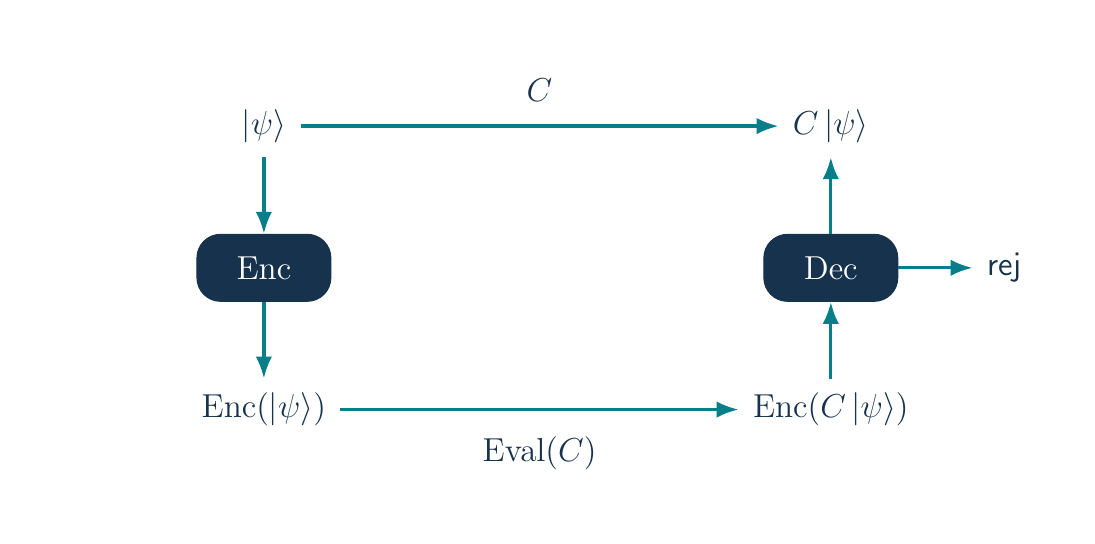
\begin{tikzpicture}[
      >={Latex[length=2.8mm]},
      state/.style={inner sep=5pt,font=\large,text=CVQCInk},
      process/.style={draw=CVQCInk,fill=CVQCInk,rounded corners=3mm,
        minimum width=1.7cm,minimum height=0.85cm,
        text=white,font=\large},
      flow/.style={->,very thick,draw=CVQCTeal},
      label/.style={font=\large,text=CVQCInk}
    ]
    \path[use as bounding box] (-6.6,-3.15) rectangle (6.6,3.05);

    \node[state] (input) at (-3.6,1.8) {$\ket{\psi}$};
    \node[state] (output) at (3.6,1.8) {$C\ket{\psi}$};
    \draw[flow] (input.east) -- node[label,above=5pt] {$C$} (output.west);

    \only<2>{
      \node[process] (enc) at (-3.6,0) {$\operatorname{Enc}$};
      \node[process] (dec) at (3.6,0) {$\operatorname{Dec}$};
      \node[state] (cipherinput) at (-3.6,-1.8)
        {$\operatorname{Enc}(\ket{\psi})$};
      \node[state] (cipheroutput) at (3.6,-1.8)
        {$\operatorname{Enc}(C\ket{\psi})$};
      \node[state] (reject) at (5.8,0) {$\mathsf{rej}$};

      \draw[flow] (input.south) -- (enc.north);
      \draw[flow] (enc.south) -- (cipherinput.north);
      \draw[flow] (cipherinput.east) --
        node[label,below=6pt] {$\operatorname{Eval}(C)$} (cipheroutput.west);
      \draw[flow] (cipheroutput.north) -- (dec.south);
      \draw[flow] (dec.north) -- (output.south);
      \draw[flow] (dec.east) -- (reject.west);
    }
  \end{tikzpicture}

  \note<1>{
    \footnotesize
    We want to apply a circuit C to the authenticated input. The top arrow
    is the desired logical computation. The pure-state, unitary notation is
    a cartoon: the authenticated computation also has to preserve correlations
    with an external reference, and our eventual application has measurements.
  }
  \note<2>{
    \footnotesize
    The lower route performs the computation while the data stays
    authenticated. For honest prescribed evaluation, decoding gives the same
    logical result as the top arrow. Enc on the right uses the updated key;
    we suppress keys throughout the picture. The verifier tracks those updates
    without revealing the key to the prover. Dec includes verification and
    can reject; the branch on the right recalls the security goal against
    deviations: the intended result or rejection, with negligible total
    accepted error. This is not an arbitrary QAS feature: we need a scheme
    and gate procedures that support authenticated evaluation. Some gates
    need interaction and auxiliary authenticated states. It is also distinct
    from the classical-client QFHE used later in the remote state preparation
    step. The next slide illustrates the particularly simple CNOT procedure
    for the trap code. The manuscript's Non-CCZ Evaluation section describes
    the operation and the verifier's key updates.
  }
\end{frame}

% Adapted from the newer reference talk's aligned-block CNOT picture.
\begin{frame}{Background: Homomorphic CNOT}
  \centering
  \begin{tikzpicture}[
      >={Latex[length=2.6mm]},
      qubit/.style={rounded corners=1.5pt,minimum width=0.56cm,
        minimum height=0.58cm,inner sep=0pt,thick},
      data/.style={qubit,draw=CVQCTeal,fill=CVQCPale},
      ztrap/.style={qubit,draw=CVQCGold,fill=CVQCGoldPale},
      xtrap/.style={qubit,draw=CVQCInk,fill=CVQCFog},
      hidden/.style={qubit,draw=CVQCMuted,fill=CVQCFog}
    ]
    \path[use as bounding box] (-6.6,-3.15) rectangle (6.6,3.05);

    \node[font=\large,text=CVQCInk] at (0.8,2.1) {Same permutation};
    \node[anchor=east,font=\large,text=CVQCInk] at (-4.05,0.75)
      {$\operatorname{Enc}(\ket{\psi})$};
    \node[anchor=east,font=\large,text=CVQCInk] at (-4.05,-0.75)
      {$\operatorname{Enc}(\ket{\phi})$};

    % Four data positions and four of each trap type; physical counts schematic.
    % The revealed colors are for the audience, not information given to the server.
    \foreach \i/\kind in {0/ztrap,1/data,2/xtrap,3/ztrap,4/data,5/xtrap,
        6/xtrap,7/ztrap,8/data,9/ztrap,10/data,11/xtrap} {
      \pgfmathsetmacro{\x}{-3.6+0.8*\i}
      \only<1>{
        \node[hidden] at (\x,0.75) {};
        \node[hidden] at (\x,-0.75) {};
      }
      \only<2>{
        \node[\kind] at (\x,0.75) {};
        \node[\kind] at (\x,-0.75) {};
      }
      \draw[thick,draw=CVQCInk] (\x,0.75) -- (\x,-0.75);
      \fill[CVQCInk] (\x,0.75) circle (2pt);
      \draw[thick,draw=CVQCInk,fill=white] (\x,-0.75) circle (0.14);
      \draw[thick,draw=CVQCInk]
        ({\x-0.14},-0.75) -- ({\x+0.14},-0.75)
        (\x,-0.89) -- (\x,-0.61);
    }

    \draw[decorate,decoration={brace,mirror,amplitude=5pt},
      thick,draw=CVQCMuted] (-3.9,-1.25) -- (5.5,-1.25);
    \node[font=\large,text=CVQCInk] at (0.8,-1.95) {Transversal CNOT};
  \end{tikzpicture}

  \note<1>{
    \footnotesize
    Take two authenticated logical qubits. The first row is the control and
    the second is the target. Both blocks use the same hidden permutation,
    with independent one-time pads. Apply a physical CNOT from each position
    in the first ciphertext to the corresponding position in the second.
    There are 3n physical CNOTs, where n is the underlying code block length;
    the twelve drawn pairs are schematic. The prover can do this without
    learning which positions contain encoded data or either type of trap.
    The verifier updates its pad keys. If the old keys are
    (x1,z1) and (x2,z2), the new keys are
    (x1,z1 XOR z2) and (x1 XOR x2,z2).
  }
  \note<2>{
    \footnotesize
    Reveal the colors only to explain why the operation works. The prover
    never learns them. Matching permutations align data with data, zero traps
    with zero traps, and plus traps with plus traps. The CSS code implements
    the logical CNOT transversally. CNOT preserves each pair of zero traps
    and each pair of plus traps, so the traps remain valid under the updated
    pad keys. The two logical output registers may be entangled; the input
    labels on the left do not assert product-form outputs. This explains
    honest correctness; security against deviations still uses authentication.
    Other gates, especially the non-Clifford resource needed for our
    computation, require additional procedures rather than just transversal
    gates. Figure adapted from the newer reference talk's Background:
    Homomorphic CNOT slide. Protocol and key update: the manuscript's
    Non-CCZ Evaluation section.
  }
\end{frame}

% Shared with the Challenges slide; optional style highlights the MBQC output.
\newcommand{\protocolflowchart}[1][]{%
  \begin{scope}[
      >={Latex[length=1.5mm,width=1.1mm]},
      stage/.style={draw=CVQCInk,fill=CVQCFog,thick,rounded corners=2mm,
        minimum width=5.6cm,minimum height=0.45cm,inner sep=2pt,
        align=center,font=\footnotesize\bfseries,text=CVQCInk},
      state/.style={inner xsep=2pt,inner ysep=1pt,
        font=\footnotesize,text=CVQCInk},
      flow/.style={->,line width=1pt,draw=CVQCTeal,
        shorten <=0.8pt,shorten >=0.8pt}
    ]
    \node[stage,fill=CVQCPale] (rsp) at (0,2.65)
      {Remote state preparation};
    \node[state] (inputs) at (0,1.85)
      {$\ket{+_{\theta}},\;\ket{0},\;\ket{1}$};
    \node[stage] (mbqc) at (0,1.05) {Verified MBQC};
    \node[state,#1] (rawmagic) at (0,0.25)
      {$\operatorname{Enc}(\ket{\mathrm{CCZ}})$};
    \node[stage] (distill) at (0,-0.55) {Authenticated distillation};
    \node[state] (cleanmagic) at (0,-1.35)
      {$\operatorname{Enc}(\ket{\mathrm{CCZ}})$};
    \node[stage] (eval) at (0,-2.15) {Evaluation};
    \node[state] (output) at (0,-2.90)
      {$y\;\text{or}\;\mathsf{rej}$};

    \draw[flow] (rsp.south) -- (inputs.north);
    \draw[flow] (inputs.south) -- (mbqc.north);
    \draw[flow] (mbqc.south) -- (rawmagic.north);
    \draw[flow] (rawmagic.south) -- (distill.north);
    \draw[flow] (distill.south) -- (cleanmagic.north);
    \draw[flow] (cleanmagic.south) -- (eval.north);
    \draw[flow] (eval.south) -- (output.north);
  \end{scope}%
}

% Show the whole pipeline immediately; only the QPIP_1 enclosure is revealed.
\begin{frame}{Protocol Overview}
  \centering
  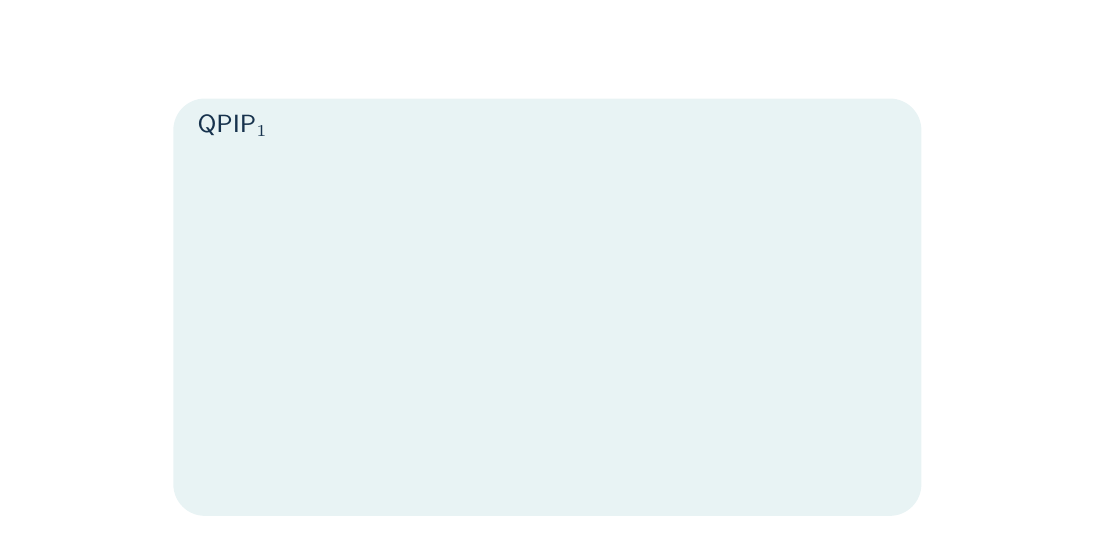
\begin{tikzpicture}[
      protocolbox/.style={draw=none,fill=CVQCPale,rounded corners=4mm},
      modellabel/.style={inner sep=0pt,
        font=\small\bfseries,text=CVQCInk}
    ]
    \path[use as bounding box] (-6.6,-3.20) rectangle (6.6,3.05);

    \only<2>{
      \path[protocolbox] (-4.75,-3.15) rectangle (4.75,2.15);
      \node[modellabel,anchor=north west] at (-4.45,1.95)
        {$\mathsf{QPIP}_1$};
    }

    \protocolflowchart
  \end{tikzpicture}

  \note<1>{
    \footnotesize
    Read the complete pipeline from top to bottom. Remote state preparation
    supplies single qubits held by the prover, with their descriptions known
    to the classical verifier. These are equatorial states with theta a
    multiple of pi/4, or computational-basis states. The parties use them
    for MBQC preparation, including hidden real and trap copies, trap checks,
    and conversion of the output pads to Pauli pads. Enc denotes trap-code
    authentication. The first CCZ label denotes the intended magic states:
    the surviving batch can still contain faults. Its joint error structure
    is the central promise to establish, not a claim that every copy is
    already correct. Authenticated distillation suppresses the remaining
    errors, then authenticated evaluation uses the distilled magic states
    to run the target sampling circuit. The final measurement and decoding
    return y, or rejection if a check fails. CCZ states stand for the full
    collection of required magic states; the picture suppresses the other
    types, multiplicities, and auxiliary distillation trees. Source: the
    manuscript's Classical Verifier Protocol section.
  }
  \note<2>{
    \footnotesize
    The box identifies our statistically secure QPIP1 protocol. A weak
    quantum verifier prepares and sends the single-qubit inputs directly;
    all later interaction is classical. The three stages inside are MBQC
    preparation and testing, authenticated distillation, and authenticated
    evaluation. The classical-verifier compilation replaces only that
    single-qubit preparation with remote state preparation, the stage above
    the box. The full compiled protocol is computationally secure; the box
    does not include the RSP assumption. This enclosure is the slide's only
    transition. Next, ask what guarantee MBQC establishes for the states
    entering distillation, and which joint input-quality promise distillation
    actually needs.
  }
\end{frame}

% Keep the overview as a map; focus on the batch passed to distillation.
\begin{frame}{Challenges}
  \centering
  \setbeamercolor{itemize item}{fg=CVQCTeal}
  \begin{tikzpicture}[>={Latex[length=2mm,width=1.4mm]}]
    \path[use as bounding box] (-6.6,-3.20) rectangle (6.6,3.05);

    \begin{scope}[shift={(-3.2,0)}]
      \path[fill=CVQCPale,rounded corners=4mm]
        (-3.4,-3.15) rectangle (3.4,2.15);
      \node[anchor=north west,inner sep=0pt,
        font=\small\bfseries,text=CVQCInk] at (-3.10,1.95)
        {$\mathsf{QPIP}_1$};
      \protocolflowchart[fill=CVQCGoldPale,rounded corners=1.5mm,
        inner xsep=5pt]
    \end{scope}

    \node[anchor=west,inner sep=0pt,text=CVQCInk] at (0.80,0.25) {%
      \begin{minipage}{5.7cm}
        \raggedright
        \begin{itemize}
          \setlength{\itemsep}{1.0em}
          \item What does MBQC guarantee?
          \item What is distillable?
        \end{itemize}
      \end{minipage}%
    };
    \draw[->,very thick,draw=CVQCTeal,shorten >=2pt]
      (0.50,0.25) -- (rawmagic.east);
  \end{tikzpicture}

  \note{
    \footnotesize
    The highlighted batch connects preparation to distillation. Ask what
    MBQC and its trap-copy tests guarantee against a malicious prover,
    and whether that joint guarantee suffices for distillation.
    Recall the earlier example verbally. With probability
    $p=1/\mathrm{poly}$, all copies may be maliciously bad together;
    otherwise all are ideal. Each marginal has error at most p, but this
    alone does not establish distillability. If that branch passes with
    constant probability and gives a wrong output, its accepted bad weight
    remains inverse-polynomial. We are not claiming every all-bad batch
    passes: reliable rejection would eliminate the branch.
    We instead need the required factorizable error structure and a joint
    bound on how many copies are bad, except for negligible accepted weight.
    Authentication addresses malicious execution; it does not certify
    correctly prepared magic states. Next, explain the MBQC preparation
    and its error structure. Keep the counterexample off the slide.
  }
\end{frame}

% The paper's brickwork graph, with the general MBQC points revealed below.
\begin{frame}{Background: Measurement-Based Quantum Computation}
  \centering
  \setbeamercolor{itemize item}{fg=CVQCTeal}
  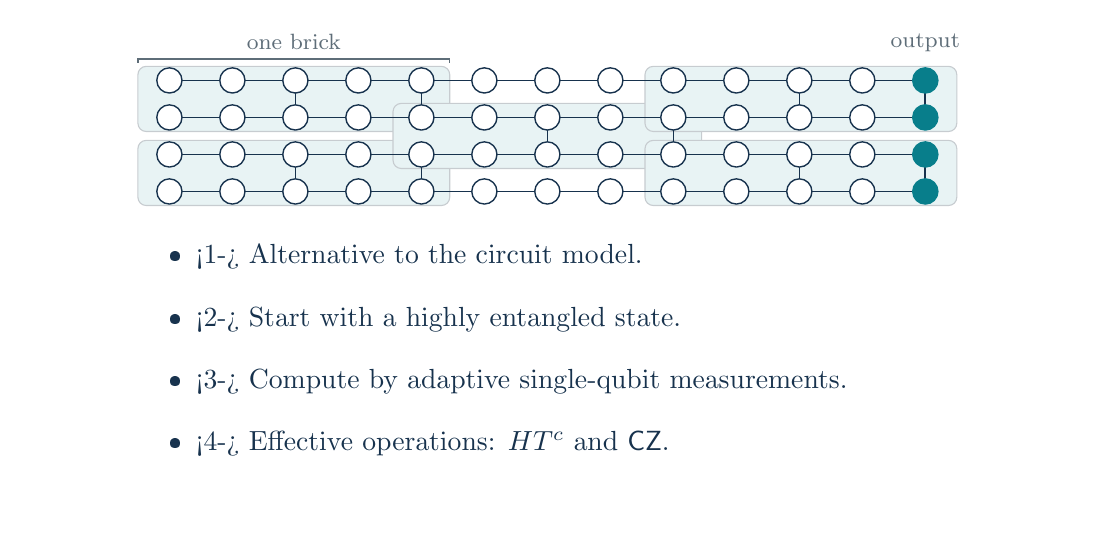
\begin{tikzpicture}
    \path[use as bounding box] (-6.6,-3.15) rectangle (6.6,3.05);

    \begin{scope}[shift={(-5.6,2.85)},x=0.8cm,y=0.47cm]
      % Topology copied from CVQC-paper/figures/brickwork_figure.tex:
% four logical rows and thirteen columns. The caller sets coordinate units.
\begin{scope}[
    qubit/.style={circle,draw=CVQCInk,line width=0.5pt,fill=white,
      inner sep=0pt,minimum size=3.2mm},
    output qubit/.style={qubit,draw=CVQCTeal,fill=CVQCTeal},
    edge/.style={draw=CVQCInk,line width=0.6pt},
    brick/.style={rounded corners=3pt,fill=CVQCPale,
      draw=CVQCMuted!35,line width=0.4pt},
    graph label/.style={font=\footnotesize,text=CVQCMuted}
  ]
  % Each shaded brick spans two rows and five columns.
  \foreach \xa/\xb/\r in {0.5/5.45/1,0.5/5.45/3,4.55/9.45/2,
      8.55/13.5/1,8.55/13.5/3} {
    \draw[brick] (\xa,{-\r+0.38}) rectangle (\xb,{-\r-1.38});
  }

  \foreach \r in {1,...,4} {
    \draw[edge] (1,-\r) -- (13,-\r);
  }
  \foreach \x in {3,5,11,13} {
    \foreach \r in {1,3} {
      \draw[edge] (\x,-\r) -- (\x,{-\r-1});
    }
  }
  \foreach \x in {7,9} {
    \draw[edge] (\x,-2) -- (\x,-3);
  }

  \foreach \r in {1,...,4} {
    \foreach \x in {1,...,12} {
      \node[qubit] at (\x,-\r) {};
    }
    \node[output qubit] at (13,-\r) {};
  }

  \draw[draw=CVQCMuted,line width=0.5pt]
    (0.5,-0.52) -- (0.5,-0.42) -- (5.45,-0.42) -- (5.45,-0.52);
  \node[graph label,anchor=south] at (2.975,-0.42) {one brick};
  \node[graph label,anchor=south] at (13,-0.5) {output};
\end{scope}

    \end{scope}

    \node[anchor=north west,inner sep=0pt,text=CVQCInk] at (-5.35,0.30) {%
      \begin{minipage}{11.2cm}
        \raggedright
        \begin{itemize}
          \setlength{\itemsep}{0.65em}
          \item<1-> Alternative to the circuit model.
          \item<2-> Start with a highly entangled state.
          \item<3-> Compute by adaptive single-qubit measurements.
          \item<4-> Effective operations: $HT^c$ and $\mathsf{CZ}$.
        \end{itemize}
      \end{minipage}%
    };
  \end{tikzpicture}

  \note{
    \footnotesize
    MBQC means measurement-based quantum computation. Show the paper's
    four-row, thirteen-column brickwork graph. Vertices are physical
    qubits and edges represent CZ entangling operations. White vertices
    are measured column by column from left to right; the teal vertices
    in the final column remain as outputs. Shaded rectangles mark the
    repeated two-row, five-column bricks. Each row carries one logical
    qubit through the computation. The prover forms this highly
    entangled graph state from individual qubits; the verifier does not
    have to prepare an entangled state.
    The computation proceeds through single-qubit measurements. Earlier
    outcomes determine later measurement bases and the corrections tracked
    by the verifier. Our effective elementary operations
    are $HT^c$, for $c\in\{0,\ldots,7\}$, and CZ. This family is universal:
    c=0 gives H, composing H with HT gives T, and CZ is entangling.
    MBQC alone does not establish blindness or verification; the encrypted
    construction and tests come later. We will return to the plaintext
    gate-teleportation example in the technical part of the talk.
    Figure source: the paper's Preliminaries, brickwork graph.
  }
\end{frame}

% Paper's fig:plaintext-mbqc, with labels for the classical and quantum outputs.
\begin{frame}{Plaintext MBQC}
  \centering
  \begin{tikzpicture}
    \path[use as bounding box] (-6.6,-3.15) rectangle (6.6,3.05);
    % Qcircuit's stick labels extend outside its measured matrix width.
    \node[inner sep=0pt,text=CVQCInk] at (-1.25,0.15) {%
      \scalebox{1.8}{%
        $\Qcircuit @C=1em @R=1em {
          \lstick{\ket{\psi}} & \ctrl{1} & \gate{HT^c} & \meter & \rstick{m}\cw \\
          \lstick{\ket{+}} & \control \qw & \qw & \qw & \rstick{X^mHT^c\ket{\psi}}\qw
        }$%
      }%
    };
  \end{tikzpicture}

  \note{
    \footnotesize
    This is the plaintext MBQC circuit from the manuscript's Technical
    Overview, Figure ``Gate teleportation.'' The input is psi on the upper
    wire and a fresh plus state on the lower wire. The two connected dots
    implement CZ. Apply $HT^c$ to the upper wire, then measure it in the
    computational basis. Equivalently, choose a measurement basis determined
    by c. Here $T=\operatorname{diag}(1,e^{i\pi/4})$ and c ranges from 0 to 7.
    If the outcome is m, the surviving lower wire holds
    $X^m HT^c\ket{\psi}$. This is the intended gate up to a known X
    correction; the upper output wire carries the classical measurement
    outcome. Repeating this gadget lets us implement gates through
    measurements, tracking corrections and adjusting later bases adaptively.
    Together with CZ, these operations are universal. The labels identify
    the classical outcome and the conditional state on the surviving wire.
    Explain the corrections in words; key updates and the encrypted version
    come later, when we introduce hiding and testing.
  }
\end{frame}

% The paper's plaintext trap example, specialized to c=0.
\begin{frame}{MBQC: Trap Copies}
  \centering
  \setbeamercolor{itemize item}{fg=CVQCTeal}
  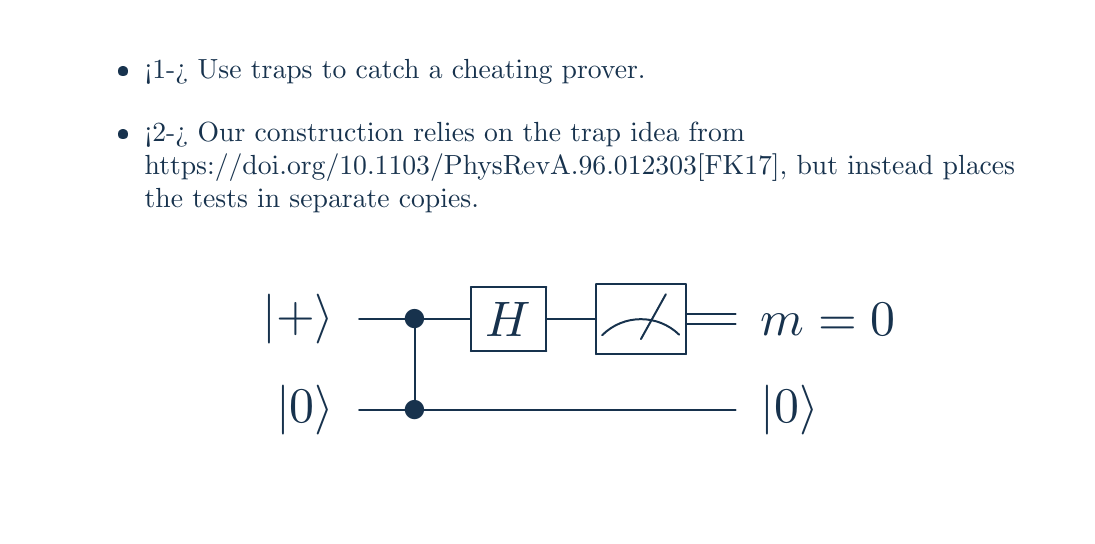
\begin{tikzpicture}
    \path[use as bounding box] (-6.6,-3.15) rectangle (6.6,3.05);

    \node[anchor=north west,inner sep=0pt,text=CVQCInk] at (-6.0,2.65) {%
      \begin{minipage}{12cm}
        \raggedright
        \begin{itemize}
          \setlength{\itemsep}{0.65em}
          \item<1-> Use traps to catch a cheating prover.
          \item<2-> Our construction relies on the trap idea from
            \href{https://doi.org/10.1103/PhysRevA.96.012303}{[FK17]},
            but instead places the tests in separate copies.
        \end{itemize}
      \end{minipage}%
    };

    \only<3>{
      \node[inner sep=0pt,text=CVQCInk] at (0,-1.05) {%
        \scalebox{1.8}{%
          $\Qcircuit @C=1em @R=1em {
            \lstick{\ket{+}} & \ctrl{1} & \gate{H} & \meter & \rstick{m=0}\cw \\
            \lstick{\ket{0}} & \control \qw & \qw & \qw & \rstick{\ket{0}}\qw
          }$%
        }%
      };
    }
  \end{tikzpicture}

  \note<1>{
    \footnotesize
    The preceding plaintext circuit explains honest computation, but a
    malicious prover may perform a different computation or lie about a
    measurement result. Introduce tests with predictable honest outcomes.
    Such traps let the verifier check the prover's reports. This is the
    motivation, not a claim that one trap detects every possible deviation.
  }
  \note<2>{
    \footnotesize
    The second bullet is copied from the manuscript's Technical Overview,
    subsection Trap Copy and Cut-and-Choose. FK17 is Fitzsimons--Kashefi,
    Unconditionally Verifiable Blind Quantum Computation (2017). Our
    construction places the tests in separate MBQC copies, using the same
    public graph and schedule as real copies. The verifier secretly chooses
    which copies to test. A trap copy uses trap and dummy vertices, with
    deterministic decoded outcomes at the checked measurements. We later
    use hidden trap copies and cut-and-choose to control the number of
    corrupted real copies; some errors can survive these tests.
  }
  \note<3>{
    \footnotesize
    This is the paper's Figure ``A plaintext trap,'' specialized to c=0.
    In the general example the upper input is $T^{-c}\ket{+}$ and the lower
    input is $\ket{0}$. Setting c=0 gives the displayed plus and zero inputs,
    and the gate $HT^0$ is H. CZ does nothing because the lower input is zero.
    H maps the upper plus state to zero, so its measurement deterministically
    returns m=0. The lower wire stays in zero. A reported result of one
    exposes a deviation. This is a test circuit with different inputs from
    the computation gadget: the lower output formula from the real example
    assumed a fresh plus state and should not be substituted here.
    The plaintext example alone does not hide the trap. Next, one-time pad
    the inputs and mask the measurement instructions, so the prover cannot
    distinguish real and trap copies and selectively attack only the real
    ones. The full trap-copy protocol uses plaintext exponent zero.
  }
\end{frame}

% Add each subsequent slide file here as we work through outline.md.

\end{document}
